% Page 5: account/matching/draw ER, including global tables.
\section{数据关系与状态设计}
\subsection{账号、匹配与抽取的数据关系}
图\ref{fig:design-er-account}从账号出发画出资料、互动、相遇和抽取记录，也列出了登录保护和历史维护相关记录。三张 ER 图共享账号实体。实线表示数据库外键，虚线表示应用层的逻辑关系。基数由父记录指向子记录，账号关联沿共用干线展开。

\begin{figure}[H]
\centering
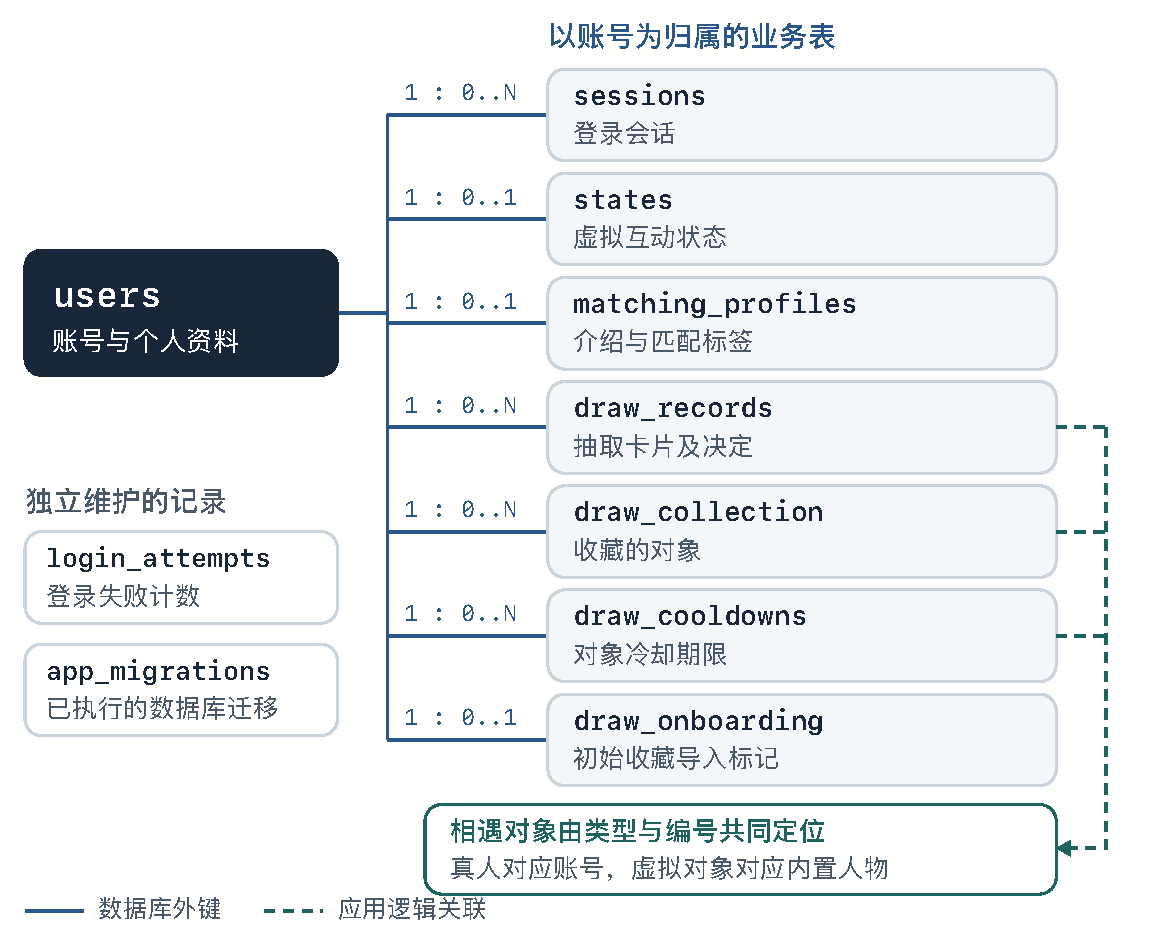
\includegraphics[width=\linewidth]{assets/design/account-matching-er.pdf}
\caption{ER 视图一：账号资料与相遇记录的归属关系}\label{fig:design-er-account}
\end{figure}

主键标识单条记录，外键标明记录归属或关联对象。一个账号最多有一份虚拟状态和一份匹配资料，相遇历史可以存多次结果。若上一张卡片仍待处理，用户再次进入会先看到这张卡。

收藏按用户分别记录，两个人可以各自收藏同一个对象。跳过后设冷却期，以减少短期内重复抽到同一对象的情况。真人和虚拟人物用同样的卡片样式，显示时按对象类型读取账号资料或内置人物资料。数据摘要见附录表\ref{tab:compact-data}。

\clearpage
